% Template for PLoS
% Version 3.5 March 2018
%
% % % % % % % % % % % % % % % % % % % % % %
%
% -- IMPORTANT NOTE
%
% This template contains comments intended 
% to minimize problems and delays during our production 
% process. Please follow the template instructions
% whenever possible.
%
% % % % % % % % % % % % % % % % % % % % % % % 
%
% Once your paper is accepted for publication, 
% PLEASE REMOVE ALL TRACKED CHANGES in this file 
% and leave only the final text of your manuscript. 
% PLOS recommends the use of latexdiff to track changes during review, as this will help to maintain a clean tex file.
% Visit https://www.ctan.org/pkg/latexdiff?lang=en for info or contact us at latex@plos.org.
%
%
% There are no restrictions on package use within the LaTeX files except that 
% no packages listed in the template may be deleted.
%
% Please do not include colors or graphics in the text.
%
% The manuscript LaTeX source should be contained within a single file (do not use \input, \externaldocument, or similar commands).
%
% % % % % % % % % % % % % % % % % % % % % % %
%
% -- FIGURES AND TABLES
%
% Please include tables/figure captions directly after the paragraph where they are first cited in the text.
%
% DO NOT INCLUDE GRAPHICS IN YOUR MANUSCRIPT
% - Figures should be uploaded separately from your manuscript file. 
% - Figures generated using LaTeX should be extracted and removed from the PDF before submission. 
% - Figures containing multiple panels/subfigures must be combined into one image file before submission.
% For figure citations, please use "Fig" instead of "Figure".
% See http://journals.plos.org/plosone/s/figures for PLOS figure guidelines.
%
% Tables should be cell-based and may not contain:
% - spacing/line breaks within cells to alter layout or alignment
% - do not nest tabular environments (no tabular environments within tabular environments)
% - no graphics or colored text (cell background color/shading OK)
% See http://journals.plos.org/plosone/s/tables for table guidelines.
%
% For tables that exceed the width of the text column, use the adjustwidth environment as illustrated in the example table in text below.
%
% % % % % % % % % % % % % % % % % % % % % % % %
%
% -- EQUATIONS, MATH SYMBOLS, SUBSCRIPTS, AND SUPERSCRIPTS
%
% IMPORTANT
% Below are a few tips to help format your equations and other special characters according to our specifications. For more tips to help reduce the possibility of formatting errors during conversion, please see our LaTeX guidelines at http://journals.plos.org/plosone/s/latex
%
% For inline equations, please be sure to include all portions of an equation in the math environment.  For example, x$^2$ is incorrect; this should be formatted as $x^2$ (or $\mathrm{x}^2$ if the romanized font is desired).
%
% Do not include text that is not math in the math environment. For example, CO2 should be written as CO\textsubscript{2} instead of CO$_2$.
%
% Please add line breaks to long display equations when possible in order to fit size of the column. 
%
% For inline equations, please do not include punctuation (commas, etc) within the math environment unless this is part of the equation.
%
% When adding superscript or subscripts outside of brackets/braces, please group using {}.  For example, change "[U(D,E,\gamma)]^2" to "{[U(D,E,\gamma)]}^2". 
%
% Do not use \cal for caligraphic font.  Instead, use \mathcal{}
%
% % % % % % % % % % % % % % % % % % % % % % % % 
%
% Please contact latex@plos.org with any questions.
%
% % % % % % % % % % % % % % % % % % % % % % % %

\documentclass[10pt,letterpaper]{article}
\usepackage[top=0.85in,left=2.75in,footskip=0.75in]{geometry}

% amsmath and amssymb packages, useful for mathematical formulas and symbols
\usepackage{amsmath,amssymb}

% Use adjustwidth environment to exceed column width (see example table in text)
\usepackage{changepage}

% Use Unicode characters when possible
\usepackage[utf8x]{inputenc}

% textcomp package and marvosym package for additional characters
\usepackage{textcomp,marvosym}

% cite package, to clean up citations in the main text. Do not remove.
\usepackage{cite}

% Use nameref to cite supporting information files (see Supporting Information section for more info)
\usepackage{nameref,hyperref}

% line numbers
\usepackage[right]{lineno}

% ligatures disabled
\usepackage{microtype}
\DisableLigatures[f]{encoding = *, family = * }

% color can be used to apply background shading to table cells only
\usepackage[table]{xcolor}

% array package and thick rules for tables
\usepackage{array}

% create "+" rule type for thick vertical lines
\newcolumntype{+}{!{\vrule width 2pt}}

% create \thickcline for thick horizontal lines of variable length
\newlength\savedwidth
\newcommand\thickcline[1]{%
  \noalign{\global\savedwidth\arrayrulewidth\global\arrayrulewidth 2pt}%
  \cline{#1}%
  \noalign{\vskip\arrayrulewidth}%
  \noalign{\global\arrayrulewidth\savedwidth}%
}

% \thickhline command for thick horizontal lines that span the table
\newcommand\thickhline{\noalign{\global\savedwidth\arrayrulewidth\global\arrayrulewidth 2pt}%
\hline
\noalign{\global\arrayrulewidth\savedwidth}}



%%  Packages added by Colin
% /* cSpell:enable */
% Symbols
\usepackage{amsmath,amssymb,url,bm}
% Formatting
\usepackage{multicol, csquotes, scrextend, color}   %, titlesec
%% Tables, Figures
\usepackage{longtable, booktabs, pdflscape, placeins, nicematrix, tikz}
\usetikzlibrary{shapes.geometric, arrows}
\tikzstyle{org} = [ellipse, minimum width=3cm, minimum height=0.75cm, text centered, draw=black]
\tikzstyle{io} = [rectangle, minimum width=3cm, minimum height=0.75cm, text centered, draw=black]
\tikzstyle{process} = [rectangle, rounded corners, minimum width=3cm, minimum height=0.75cm, text centered, draw=black]
\tikzstyle{arrow} = [thick,->,>=stealth]

% Images
\usepackage{graphicx, float, caption, subcaption}

% package added by Oster for editing
\usepackage{color} 
\newcommand{\red}[1]{{\color{red}{#1}}}





% Remove comment for double spacing
%\usepackage{setspace} 
%\doublespacing

% Text layout
\raggedright
\setlength{\parindent}{0.5cm}
\textwidth 5.25in 
\textheight 8.75in

% Bold the 'Figure #' in the caption and separate it from the title/caption with a period
% Captions will be left justified
\usepackage[aboveskip=1pt,labelfont=bf,labelsep=period,justification=raggedright,singlelinecheck=off]{caption}
\renewcommand{\figurename}{Fig}

% Use the PLoS provided BiBTeX style
% Colin commented this out - added where bibliography is inserted
% \bibliographystyle{plos2015}

% Remove brackets from numbering in List of References
\makeatletter
\renewcommand{\@biblabel}[1]{\quad#1.}
\makeatother

% Header and Footer with logo
\usepackage{lastpage,fancyhdr,graphicx}
\usepackage{epstopdf}
%\pagestyle{myheadings}
\pagestyle{fancy}
\fancyhf{}
%\setlength{\headheight}{27.023pt}
%\lhead{\includegraphics[width=2.0in]{PLOS-submission.eps}}
\rfoot{\thepage/\pageref{LastPage}}
\renewcommand{\headrulewidth}{0pt}
\renewcommand{\footrule}{\hrule height 2pt \vspace{2mm}}
\fancyheadoffset[L]{2.25in}
\fancyfootoffset[L]{2.25in}
\lfoot{\today}

%% Include all macros below

\newcommand{\lorem}{{\bf LOREM}}
\newcommand{\ipsum}{{\bf IPSUM}}

%% END MACROS SECTION


\begin{document}
\vspace*{0.2in}

% Title must be 250 characters or less.
\begin{flushleft}
{\Large
\textbf\newline{Prediction of first-time homelessness risk based on utility payment history} % Please use "sentence case" for title and headings (capitalize only the first word in a title (or heading), the first word in a subtitle (or subheading), and any proper nouns).
}
\newline
% Insert author names, affiliations and corresponding author email (do not include titles, positions, or degrees).
\\
Colin D.\ Middleton\textsuperscript{1\P},
Kim\ Boynton\textsuperscript{2\&},
David\ Lewis\textsuperscript{3\&},
Andrew M.\ Oster\textsuperscript{1\P*}\\

\bigskip

\textbf{1} Department of Mathematics, Eastern Washington University, Cheney, Washington, United States of America \\
\textbf{2} Avista Utilities, Spokane, Washington, United States of America \\
\textbf{3} Homeless Management Information System, City of Spokane, Spokane, Washington, United States of America \\
\bigskip


% Current address notes
%\textcurrency Current Address: Dept/Program/Center, Institution Name, City, State, Country % change symbol to "\textcurrency a" if more than one current address note
% \textcurrency b Insert second current address 
% \textcurrency c Insert third current address

% Deceased author note
%\dag Deceased

% Group/Consortium Author Note
%\textpilcrow Membership list can be found in the Acknowledgments section.

% Use the asterisk to denote corresponding authorship and provide email address in note below.
*aoster@ewu.edu

\end{flushleft}
% Please keep the abstract below 300 words
\section*{Abstract}
In this work, we present a logistic regression model that predicts risk of first known homelessness based on monthly de-identified residential utility customer billing data. This model was fitted using records from 91,591 utility primary account holders over a five year period with the method of K-Folds ($k=10$), oversampling the positive (minority) class, and scaling all features to range [0, 1]. At the prediction binning threshold of 0.407 the model achieved a True Positive Rate (Recall) of 0.899, a False Positive Rate of 0.522, and a Positive Predictive Value (Precision) of 0.007, which is commensurate with existing research. This study aims at predicting first-time homelessness based on data available on the general public where nearly all precedent research focuses on predicting chronic homelessness based on individuals already seeking assistance.

\section*{Introduction}
In order to reduce homeless numbers in Spokane County, the City of Spokane, Avista Utilities, Urbanova, Eastern Washington University and Washington State University formed a consortium, the Spokane Predictive Analytics Group, to aggregate data and develop new predictive tools to identify those at risk of homelessness. This paper is a result of the efforts of this group and the modeling approach presented here is generalizable to anywhere in the United States.

\subsection*{Background}
% Definition of Homelessness
The United States Department of Housing and Urban Development (HUD) defines categories of homelessness with their \textit{``Category 1: Literally Homeless"} as
\begin{displayquote}[\cite{hud_hmls_def}]
1) Individual or family who lacks a fixed, regular, and adequate nighttime residence, meaning: \\
(i) Has a primary nighttime residence that is a public or private place not meant for human habitation; \\
(ii) Is living in a publicly or privately operated shelter designated to provide temporary living arrangements (including congregate shelters, transitional housing, and hotels and motels paid for by charitable organizations or by federal, state and local government programs); or \\
(iii) Is exiting an institution where (s)he has resided for 90 days or less and who resided in an emergency shelter or place not meant for human habitation immediately before entering that institution
\end{displayquote}

The agencies that collected the data utilized in this work used HUD's \textit{``Category 1: Literally Homeless"} definition of homeless. To be consistent with the data, we adopt that definition.

\subsubsection*{The current state of homelessness}
Homelessness in the United States persists despite the efforts of various homelessness assistance programs. There has been a decrease of 42\% in homelessness in the U.S. from 2005 until 2020 according to the Department of Housing and Urban Development (HUD), but over 442,000 people were still recorded as experiencing homelessness in 2020 through HUD's Point in Time (PIT) count program~\cite{PITcount}. Local groups that perform PIT counts gather information from shelter programs and visit homeless camps counting people. These methods likely miss some people experiencing homelessness who are not present in the locations where counting is performed, but the PIT counts provide the best and most consistent data available. In Washington State, homelessness has decreased by 28\% from 2005 to 2020, but 17,264 people were still reported experiencing homelessness in 2020~\cite{PITcount}.

In this work, we consider homelessness in Spokane County, Washington, USA.  Spokane County has seen homelessness levels decrease by 32\% from 2005 to 2020 with 1,244 people recorded as experiencing homelessness in 2020. These numbers include individuals sheltered in emergency shelters, sheltered in transitional housing, and unsheltered~\cite{PITcount}. The rates of homelessness at the national, state, and county level are displayed in Fig~\ref{fig:homelessness_counts}.

\begin{figure}[!h]
    \centering
    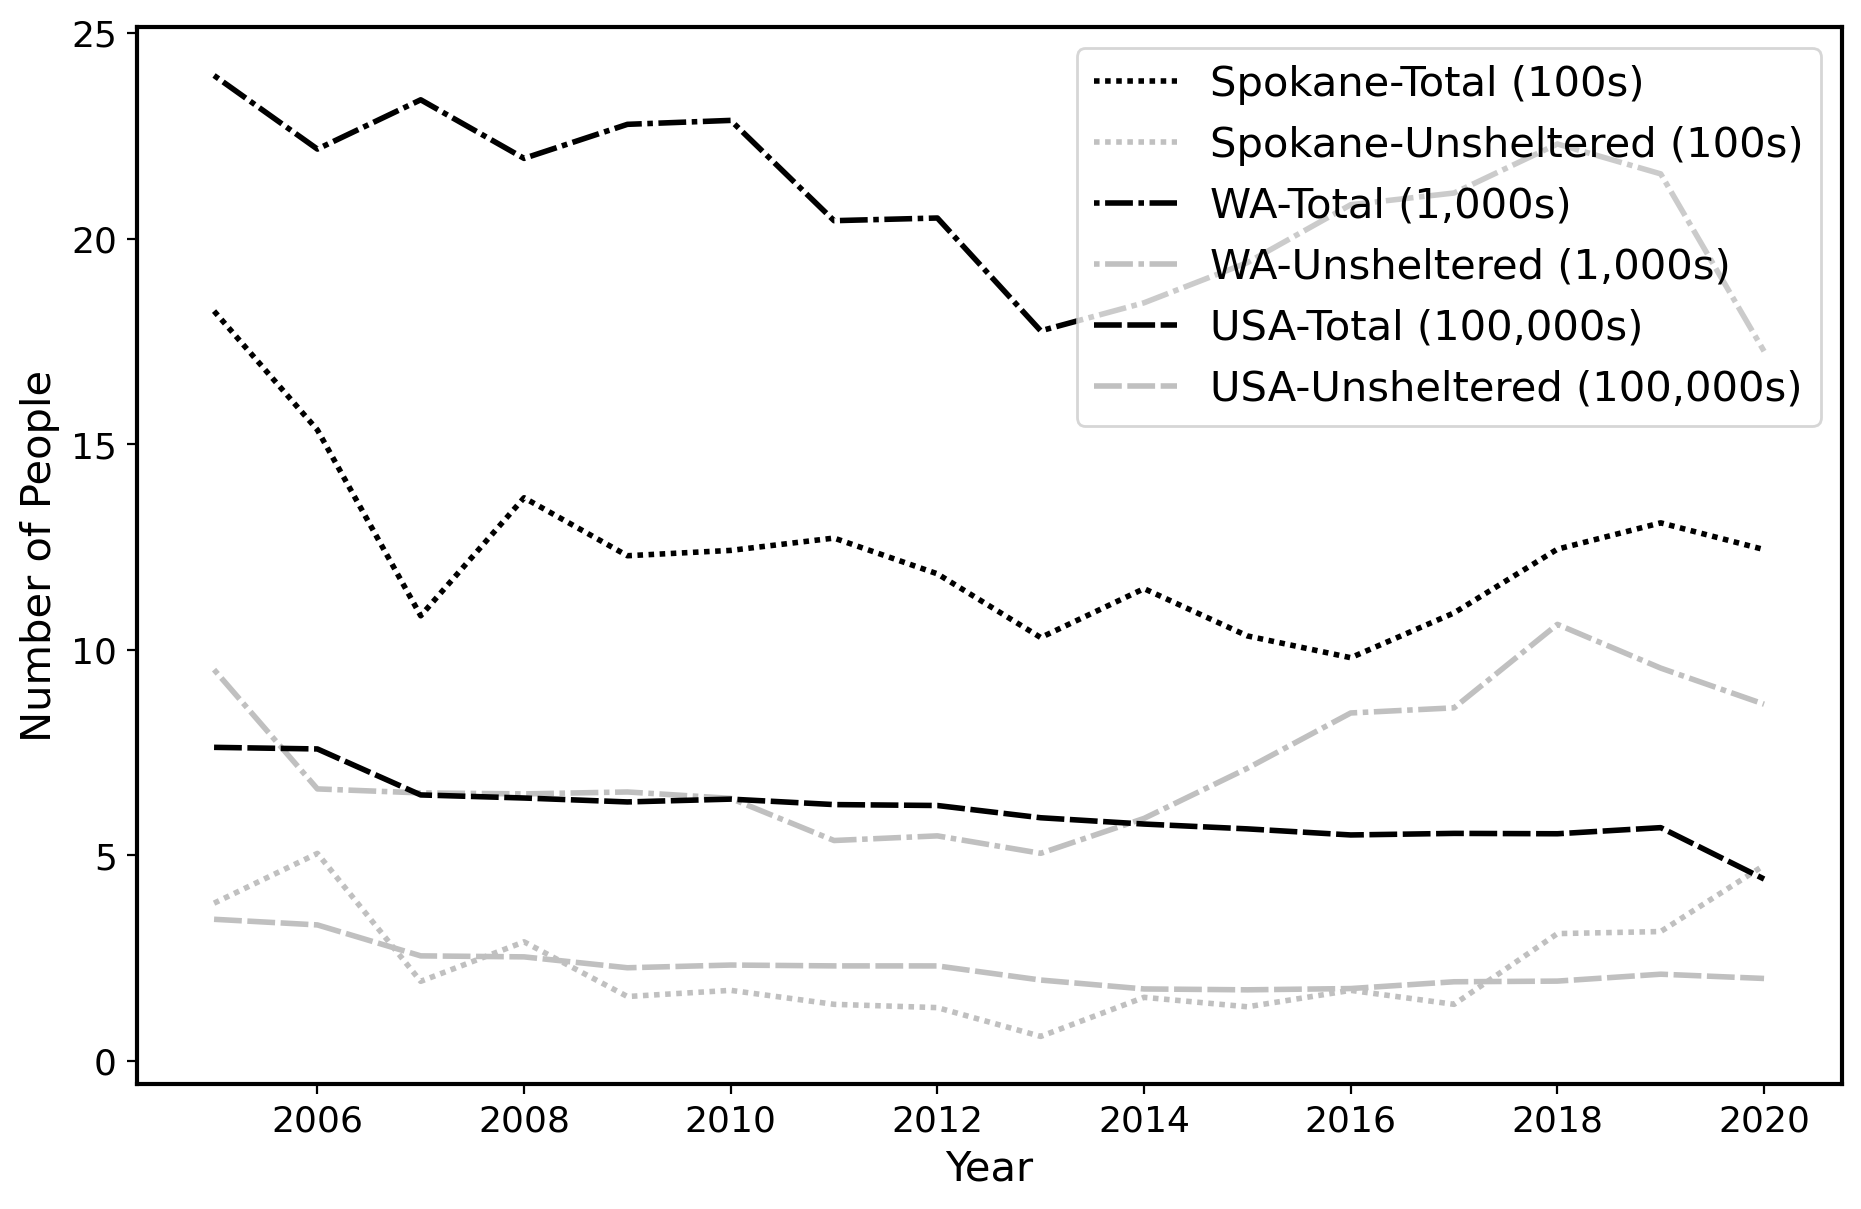
\includegraphics[width=\textwidth]{Fig1.png} %TODO: REMOVE BEFORE SUBMISSION
    \caption{{\bf Annual homelessness counts.} The counts for Spokane County (Spokane) are displayed in 100s, the counts for Washington State (WA) are displayed in 1000s, and the counts for the United States of America (USA) are displayed in 100,000s.~\cite{PITcount}}
    \label{fig:homelessness_counts}
\end{figure}

% Efforts to combat homelessness
Programs focused on providing assistance to people experiencing homelessness are having an impact. HUD's January 2019 survey found that ``there were 144,000 more permanent supportive housing (PSH) beds dedicated to people with chronic patterns of homelessness than there were in 2007 (a 380\% increase)''~\cite{2019AHAR}. Likely because of this increase in resources, the rate of chronic homelessness (people who have experienced homelessness for at least 12 months in the last three years) has declined by 20\% from 2007 to 2019 in the U.S.~\cite{2019AHAR}. Current assistance programs and the positive impacts they have on people in need represent a significant accomplishment, but these programs largely focus on providing support to people already experiencing homelessness. In order to substantially reduce and eventually end homelessness altogether, homelessness prevention programs must be utilized. 

We will refer to programs as homelessness prevention programs (HPPs) if they focus on preventing people from experiencing homelessness. These programs include permanent deep rental housing subsidies, eviction prevention programs, community based services such as short term financial assistance, education, and job placement. Homeless assistance programs (HAPs), instead, are aimed at assisting people who are currently experiencing an episode of homelessness and include shelters and other emergency services. 

There are two aspects of HPPs that make them more attractive than HAPs. The first is cost. The services that HPPs typically offer are less expensive for taxpayers than those provided by HAPs~\cite{shinn2019homelessness}. The second is that if an HPP is successful, it spares people the trauma typical of experiencing homelessness.

\subsubsection*{Cost-effectiveness of homelessness prevention programs}
Research has shown that many types of HPPs are cost-effective in practice, meaning that treating the socioeconomic issue of homelessness with HPPs instead of HAPs is at least as effective at keeping people off the streets and requires less expenditure than HAPs. This is due to the high cost of the financial health and mental health rehabilitation services HAPs must provide. Once someone experiences an episode of homelessness, in order to effectively rehabilitate that individual, they may require housing assistance, financial assistance, and mental health counseling.

A study on permanent deep rental housing subsidies, one of the most promising types of HPP, found that ``among the 67 percent of families who successfully used their [rent subsidy] voucher to lease housing, homelessness was prevented entirely''~\cite{shinn2019homelessness}. Another study analyzed an eviction prevention program from 2010 to 2012 in Chicago that distributed rent assistance based on at-risk individuals calling a Homelessness Prevention Call Center. Researchers found that ``the volatile nature of funding availability leads to good-as-random variation in the allocation of resources to individuals seeking assistance'' and that ``those calling when funding is available are 76\% less likely to enter a homeless shelter''~\cite{evans2016impact}. The program was especially helpful for the lower-income callers, and, the authors claim, could have been more efficient with better targeting of this group~\cite{evans2016impact}. In New York City a program called Homebase provides community based services to at-risk individuals. Two studies have concluded that this program is cost-effective at preventing homelessness~\cite{rolston2013evaluation, goodman2016homelessness}.

Homeless prevention is effective on a large scale as well. In 2009 the United States government distributed \$1.5 billion through the Homeless Prevention and Rapid Rehousing Program which promoted HPPs. According to the National Alliance to End Homelessness this support of HPPs largely drove the 1\% decline in homelessness between 2009 and 2011, which is notable considering the economic recession during that time~\cite{shinn2013efficient}.

% The pathology of homelessness
There is an important pattern in the pathology of homelessness that is likely the cause of HPPs' effectiveness - a gradual and measurable divergence from financial stability. We hypothesize that individuals that eventually experience homelessness begin their journey as indistinguishable from the healthy population, but, as time moves forward, these individuals begin to show signs of financial distress and become more and more separate from the financially healthy population (and more identifiable as at-risk) as they progress towards experiencing homelessness. As this progression continues, and especially once an individual experiences an episode of homelessness, it becomes more difficult to change their financial trajectory and help them reestablish their financial independence. This hypothesis is supported by Shinn et al., who found that ``[t]he single best predictor of eventual homelessness is having previously been in a shelter''~\cite{shinn2019homelessness}. The benefit of HPPs is that they endeavor to change the trajectories of at-risk individuals early in their progression towards homelessness. If an intervention is performed early, only a minor, inexpensive course correction is necessary. 

If this process is allowed to progress too long, especially if an individual experiences homelessness, the required intervention is much more costly. Evans et al. found, using the Homelessness Prevention Call Center mentioned previously, that ``[t]he per-person cost of averting homelessness through financial assistance is estimated as \$10,300 and would be much less with better targeting of benefits to lower-income callers. The estimated benefits, not including many health benefits, exceed \$20,000''~\cite{evans2016impact}. A 2019 report published by the Economic Roundtable focused on predicting persistent homelessness states, ``The longer people are homeless, the worse their problems become, making it more difficult and expensive to stably house them''~\cite{toros2019early}. This indicates that prevention, using HPPs, is far less expensive than waiting to assist people with HAPs only after they have experienced an episode of homelessness.

% No one is too high-risk to assist
One concern with HPPs is if there are portions of the population that would not benefit from assistance. In a study on New York's HomeBase program in 2013 it was found that ``[n]o level of risk was too high for families to benefit from services and, indeed, even in the highest decile of measured risk, a majority of families avoided shelter''~\cite{shinn2013efficient}. This finding provides statistical backing to the notion that no one is beyond help. It also informs which part of the population HPPs should focus on: people who are predicted to have the highest risk of experiencing homelessness. This portion of the population is most likely to experience homelessness, according to the prediction model, and will still benefit from assistance.

% Large net vs small net
According to a 2019 study by the California Policy Lab, HPPs should be both effective and efficient. An entirely \textit{effective} program prevents all people from experiencing homelessness and an entirely \textit{efficient} program provides assistance only to those who would experience homelessness if unassisted~\cite{von2019predicting}. A useful analogy is that HPPs striving to provide assistance to a certain type of person, those who will experience homelessness, is like casting a net to catch a certain type of fish. Programs that ``cast a large net'' by assisting many people can easily be effective because they are likely to prevent a large number of people from experiencing homelessness. However, it is difficult for such a program to be efficient because it will inevitably provide assistance to many people who would not experience homelessness even if they did not receive assistance. Similarly, a program that ``casts a small net,'' targeting the people identified as most at-risk of experiencing homelessness, can be highly efficient by only providing assistance to people who would have experienced homelessness, but is likely less effective because some people who do not receive assistance will still experience homelessness simply because they were not identified as the most at-risk. The ideal situation is a program that assists all the people who would experience homelessness and none who would not. This ideal is almost certainly unattainable in practice due to the difficulty of identifying who will experience homelessness, but HPPs can still strive to achieve high effectiveness and efficiency. The key to providing this targeted assistance is correctly identifying the most at-risk individuals and doing so as early as possible in order to give them the best chance at correcting their financial trajectories.

\subsubsection*{Predicting homelessness}
Identifying individuals to enroll in HPPs is a difficult task because everyone is a candidate; anyone might experience homelessness at some point in the future. The path to homelessness may be different for different individuals and people may persist in a high-risk-of-homelessness state without ever experiencing an episode of homelessness. Only when a tipping point is reached - too many bills are due at once or an unforeseen expense is incurred such as a parking ticket or a medical expense - does someone lose their ability to retain housing and experience an episode of homelessness~\cite{o2004wrong}. Because of this ability for some individuals to maintain a state of financial instability but never experience homelessness, even the best prediction models will likely produce false positives, that is, predict some people as having a high risk of experiencing homelessness when they never actually experience homelessness.

Currently, screening for HPPs is almost entirely performed by healthcare workers. Using surveys, their experience, and their intuition they evaluate each individual and determine who gets which aid and how much. There are at times high volumes of individuals seeking assistance, especially in large cities, which slows down this system. Another issue is that the evaluators have biases which may affect their decisions about who gets aid and who does not~\cite{shinn2019homelessness}.

The use of statistical models as a screening method shows promise in this area. Statistical models add more objectivity to the screening process; any bias they contain can be measured and corrected. One study found that the use of a statistical model for applicant screening reduced the number of false negatives from 28.4\% to 8.1\%~\cite{shinn2019homelessness}. Screening systems using statistical models are easily automated, reducing the burden on healthcare workers, are less expensive to operate, and are much faster than their human equivalent, speeding up the overall process of providing assistance to those in need.

\subsection*{Project goals}
The Spokane Predictive Analytics Group was tasked with determining if utility customer billing data is useful for predicting general homelessness and to develop predictive tools to identify those at risk of homelessness within Spokane County. This paper focuses on predicting first-time homelessness at the population level. The main goal of this study is to determine if ubiquitous information contained in residential utility customer billing data is useful in predicting first-time homelessness. We accomplish this objective by using some of this data that is locally available, but could be found anywhere across the United States, to train a statistical model and predict first-time homelessness, then evaluate the model's performance. The intent is to eventually incorporate this utility data, if useful, into a larger model that pulls from other data sources. The prediction model, itself, is a secondary objective. Without incorporating any additional data, the model can be used to predict homelessness, though the performance would likely increase with additional data.

The output from the model, either the model presented in this work based solely on utility data or the intended larger model, should be easy to use by any HPP. A convenient model output format for this use-case is a list of individuals ranked by their predicted risks of experiencing homelessness. With this output format, the HPP using the model can assist at-risk individuals in two convenient ways:

\begin{itemize}
    \item Option 1
    \begin{enumerate}
        \item Assess the pool of resources available to assist at-risk individuals.
        \item Determine the number of people that can receive aid based on this pool, say $n$.
        \item Assist the $n$ individuals with the highest predicted risk.
    \end{enumerate}
    \item Option 2
    \begin{enumerate}
        \item Analyze the list of individuals and their risks of experiencing homelessness.
        \item Choose a threshold risk value.
        \item Assist all individuals above that threshold.
    \end{enumerate}
\end{itemize}

Both of these options are convenient for HPPs and can be pursued using the list of individuals ranked by their predicted risk of experiencing homelessness. The second option may be appropriate if there is a large gap in predicted risks.

\subsection*{Precedent research}
% Outcomes
All previous relevant studies found by the authors focus on predicting shelter reentry~\cite{hong2018applications}, chronic or persistent homelessness~\cite{vanberlo2021interpretable, toros2019early}, general homelessness or shelter entry~\cite{byrne2020classification, shinn2013efficient}, or costs relating to homelessness~\cite{flaming2011crisis}, not first-time homelessness. There are two likely reasons for this: justification to the public, and availability of relevant data.

One issue with preventing homelessness is the justification for spending to the public. Why spend taxpayer money to assist someone who is not experiencing homelessness? Resistance to HPPs is likely reduced when the people receiving assistance have repeatedly experienced homelessness. The main reason why previous studies have not focused on predicting first-time homelessness is likely the lack of data on the target population. In predicting first-time homelessness everyone in the general population is a potential candidate, so models need data on the entire population. Only one study was able to obtain such data: Byrne et al. predicted on ``5,050,639 [p]ersons aged 11 years or older who had health insurance between 2011 and 2015 as reported in the Massachusetts All-Payer Claims Database (APCD),'' accounting for 98\% of Massachusetts state residents, in their 2020 study~\cite{byrne2020classification}. The predictors used from this database were related to: mental health, substance abuse, emergency medical service use, incarceration, veteran status, mother's occupation, and others~\cite{byrne2020classification}. This type of data is difficult to gain access to and is not uniformly available across the United States. A national database of this kind would radically improve the ability to predict and prevent negative socioeconomic outcomes such as homelessness.

% Data sources + prediction population
Other studies predicted over subpopulations that had data relevant to homelessness similar to the study by Byrne et al. A 2011 study by Flaming et al. predicted the cost level of individuals experiencing homelessness who are seeking medical assistance or are incarcerated~\cite{flaming2011crisis}. Their goal was to identify and assist the highest cost individuals experiencing homelessness, saving the taxpayers the most money with each individual provided aid~\cite{flaming2011crisis}. A 2008 paper by Hong et al. predicted two binary outcomes, shelter reentry and if the length of shelter stay will be more than nine months, from 6,000 families served by Women-in-Need (WIN) homeless shelters in New York City~\cite{hong2018applications}. A 2013 study by Shinn et al. predicted shelter entry on ``11,105 families with incomes less than 200\% of the federal poverty level who applied for Home-Base prevention services from the New York City Department of Homeless Services between October 1, 2004, and June 30, 2008''~\cite{shinn2013efficient}. A 2019 report to the Economic Roundtable by Toros et al., mentioned previously, predicted persistent homelessness on ``over one-million residents of Los Angeles County who were homeless sometime within a 15-year window. These individuals received some type of public benefits during this period: Medi-Cal, food stamps/SNAP, CalWORKs cash aid, or General Relief cash aid''~\cite{toros2019early}. And finally, a 2020 study by VanBerlo predicted ``if clients were at risk of becoming or continuing to be chronically homelessness 6 months in the future'' over 6,521 individuals recorded in the Homeless Individuals and Families Information System of the City of London, Canada~\cite{vanberlo2021interpretable}. These studies focused on their particular subpopulations because data relevant to homelessness was available on them. In order to predict first-time homelessness, data available on the general population must be used.

% Models used
These studies either used statistical models or machine learning approaches to predict binary outcomes related to homelessness. Of the statistical models all were logistic regression~\cite{byrne2020classification,flaming2011crisis,hong2018applications,toros2019early} except Shinn et al. used Cox Proportional Hazards~\cite{shinn2013efficient}. The study by VanBerlo et al. used a complex machine learning model composed of one Long-Short Term Memory layer and seven densely connected neural network layers~\cite{vanberlo2021interpretable}. 

% Variation in performance reporting
An issue with related research to date is the non-standardized reporting of model performance. There are a variety of performance metrics for binary classification tasks such as this and the choice of which metrics to calculate and report depends on the focus of the study. In the context of predicting homelessness, research is unified in the effort to reduce false negatives with the secondary goal of reducing false positives. ``While additional services rarely will create hardship for the recipient, misallocating limited resources can have serious consequences for constrained shelter providers. More concerning, then, are false negatives, which would mean that those most at-risk are left unsupported. Given the potential impact of this type of oversight, we evaluate and tune our models to maximize recall or sensitivity [aka True Positive Rate], thereby reducing the potential false negative rate. The trade-off here, however, is an increase in the false positive rate''~\cite{hong2018applications}. VanBerlo's team reached a similar conclusion, stating that they ``considered false negatives to be more harmful than false positives and therefore throughout the study, the goal was to train a proficient model that primarily minimized false negatives, while balancing a desired decrease in false positives''~\cite{vanberlo2021interpretable}. Even with a clear focus on minimizing false negatives, studies reported a variety of performance metrics with the result of difficult model comparison. \red{remove previous paragraph?}

%------------------- Materials and Methods ---------------------------------
\section*{Materials and methods}
\subsection*{Data}
% Sources
The data used for this project was obtained from Avista Utilities and the City of Spokane. Avista Utilities provided monthly residential utility customer billing information for electricity and natural gas utilities. The City of Spokane provided monthly combined water, sewer, and garbage utility billing information as well as outcome data on who has been recorded as experiencing homelessness each month from their Community Management Information System (CMIS), which complies with HUD's Homeless Management Information System regulations. Utility billing data is attractive for two key reasons. First, it contains information related to individuals' financial health such as utility bill amounts, amount owed to the utility company, and number of times a bill payment was missed. Risk of homelessness is hypothesized to be closely linked with an individual's financial health.

The second reason why utility data is attractive is its ubiquity. Almost all households pay some form of utility bill, so this data is available for at least one member of nearly every household across the United States. This data may exist in different forms and in different agencies, but similar information on amounts owed and payment default likely exist in all residential utility-customer situations. This means that our derived model could be used anywhere in the U.S. using similar data sources.

% Data Makeup
After the preprocessing steps described below, the data covers 96,768 Avista billing accounts, 64,728 locations (premises) in Spokane County, and 91,591 people (357 positive cases and 91,234 negative cases) - about 17.5\% of Spokane County residents based on the 2019 U.S. Census~\cite{SpokanePop}. The timeframe the data covers is from December 2015, through December 2020. Prior to December 2015, Avista used a different account tracking system, and it would have been difficult to combine data from both systems. 

% Data Imbalance
The high degree of imbalance in the dataset, that is, the large number of negative cases, people who were never recorded as experiencing homelessness within the dataset, compared to the small number of positive cases, people who were recorded as experiencing homelessness, is a challenge to predicting homelessness on the population scale. Specifically, positive cases make up only 0.39\% of the people represented in the dataset. This imbalance adds difficulty to the model's task of distinguishing between positive and negative cases because it is difficult to identify the few positive cases among the many negative cases, especially if there are many negative cases that are similar to the positive cases. As indicated by previous research, correctly identifying positive cases is much more important than negative cases.

\subsubsection*{Data preparation}
% Matching + De-Identifying
A diagram of data preprocessing is displayed in Fig~\ref{fig:preprocessing} that captures the following description. Initial data matching and de-identifying was performed by the data team at Avista Utilities. This process involved joining the utility billing data from Avista and the City of Spokane on address and month. This dataset was then joined to the City of Spokane's CMIS homelessness data where matching was based on the last four digits of social security number. After matching, the data was de-identified by replacing any identifiable characteristics of the data such as name and address with internally generated identification numbers.

\begin{figure}
    \centering
    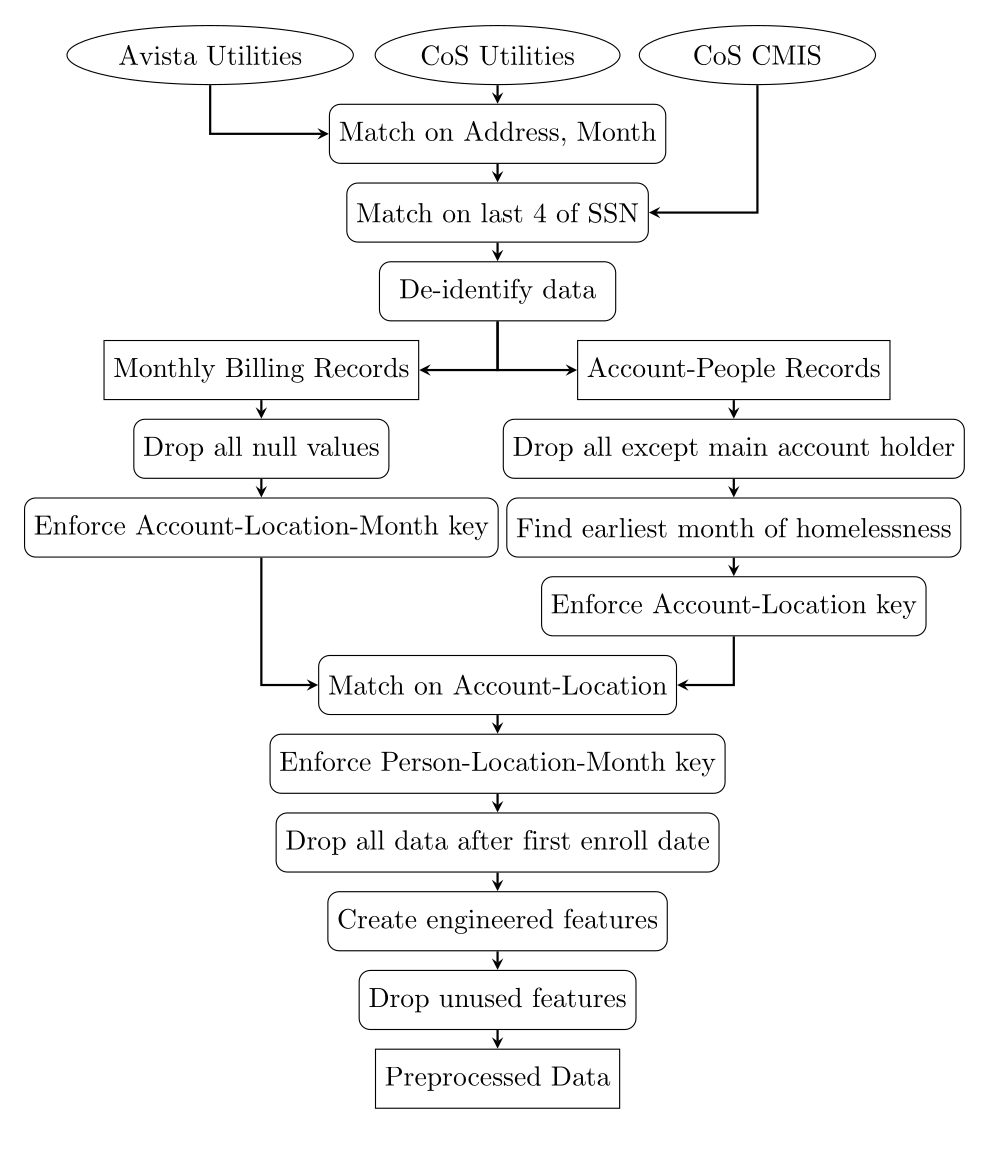
\includegraphics[width=0.9\textwidth]{Fig2.png} %TODO: REMOVE BEFORE SUBMISSION
    \caption{{\bf Data preprocessing diagram.} Initial data is provided by Avista Utilities, the City of Spokane Utilities department (CoS Utilities), and the City of Spokane CMIS that tracks homelessness (CoS CMIS). The authors received the data as two file groups, Monthly Billing Records and Account-People Records, after de-identification and initial matching was performed by the Avista data team.}
    \label{fig:preprocessing}
\end{figure}

% Account Centric -> People Centric
At this stage the utility billing activity was tied to utility customer accounts, not individual people, and each account had one or more people associated with it. All accounts had at least one (main) account holder, but many had additional parties associated with them: cotenants, landlords, third party family members, and third party agencies that could assist in bill payment. The modeling task in this context is clearly people-centric, meaning the trained model should take as input a single person's billing information and output their predicted likelihood of experiencing homelessness. This required the data be reconfigured from account-centric to people-centric. To achieve this only the main account holder was associated with each account's billing activity and all other people associated with the account were removed. If a person was associated with more than one account for the same month, one account was chosen at random to associate with the person for that month. After preprocessing the data had a composite key of person-place-month (SPA\_PER\_ID, SPA\_PREM\_ID, MONTH).

% Association Metrics + Predictor Variables
Only the variables that were most related to the outcome of homelessness and believed to be widely available across the U.S. were retained for model fitting. Point-Biserial Correlation was used to measure the strength of relationships between predictor variables and the chosen binary outcome of whether a person ever experiences first-time homelessness. Other measures of association were used for other potential outcome variables discussed in the Discussion Section. Because this modeling task focuses on prediction, intercorrelation between predictor variables was largely ignored. The short list of predictor variables used for model fitting and their definitions is shown in Table~\ref{tbl:varsUsed}. The variable BREAK\_ARRANGEMENT can be interpreted as the number of times a person has established a service break arrangement with the utility company.

\begin{table}[!h]
    \centering
    \begin{tabular}{m{4.5cm} | m{7cm}}
        \toprule
        Variable (Feature) &                  Description \\
        \hline \hline
        SPA\_PER\_ID & Unique identifier for each person. \\
        \midrule
        SPA\_PREM\_ID & Unique identifier for each location (premises). \\
        \midrule
        MONTH & Month for which data was recorded. \\
        \midrule
        CMIS\_MATCH & The binary outcome: If a person is ever recorded experiencing homelessness or not. \\
        \midrule
        PAST\_DUE & Bill past due notice sent to customer. \\
        \midrule
        TOTAL\_CUR\_BALANCE & Combined amount owed by an individual in all utilities (electirc, gas, water, sewer, garbage) on the current month. \\
        \midrule
        BREAK\_ARRANGEMENT & Service severance begun - break arrangement established for customer. \\
        \midrule
        NUM\_PER\_FOR\_PREM & Cumulative count of unique individuals recorded at a specific location (premises). \\
        \midrule
        NUM\_PREM\_FOR\_PER & Cumulative count at each month of unique locations (premises) recorded for a specific person. \\
        \bottomrule
    \end{tabular}
    \caption[Variables Used]{Variables used in model fitting and their descriptions.}
    \label{tbl:varsUsed}
\end{table}

\subsubsection*{Feature engineering}
Additional information was extracted by engineering new features not provided in the original data. The amount owed by each person at the start of each month, TOTAL\_CUR\_BALANCE, was initially provided as three separate attributes: amount owed to Avista in electricity bills, amount owed to Avista in gas bills, and amount owed to the City of Spokane in the combined bill amounts for water, sewer, and garbage. To make the variables used more closely resemble those that might be available in other utility-customer situations, the amounts owed were aggregated into a single attribute, TOTAL\_CUR\_BALANCE, representing total amount owed to all utility entities. This combined amount was more strongly correlated with the outcome of homelessness than any of the individual amounts owed.

The cumulative number of utility account holders who have lived at each location over time was calculated and recorded as NUM\_PER\_FOR\_PREM. This variable relates to the number of people who have moved away from each location and is an indicator of a mismatch between the tenant's desire and ability to live at that location. The housing may be desirable to the tenant, but they are forced to move because they cannot afford to stay either because their financial situation has deteriorated or the rent has increased. The housing may also be undesirable to the tenant and their stay was intended to be temporary from the start, in which case moving away would indicate an improvement in financial health. People move for other reasons besides the housing desirability and their ability to pay rent, but this variable was intended to capture some of that information.

The cumulative number of locations where an individual has paid utility bills over time was also calculated and recorded as NUM\_PREM\_FOR\_PER. This variable captures the number of places each person has lived, though some people pay utilities at multiple premises for reasons other than moving; they may own multiple properties or pay someone else's utility bills. This variable only captures locations where an individual is a main account holder because only main account holders were retained, so people that move and are no longer the main account holder are not captured by this variable.

\subsection*{Model}
We used multivariable binary logistic regression to predict risk of experiencing first time homelessness. This type of model has been used for predicting risk of homelessness in several previous studies~\cite{byrne2020classification,van2009longitudinal,flaming2011crisis, hong2018applications,toros2019early} and fits the situation of predicting the likelihood of a binary event based on a set of continuous predictors. For each set of new person's data fed into the model, the model will produce an output of the predicted probability an event will occur given the variable values for that person. This matches the intended use-case for the model. 

In the context of this project, the logistic regression model treats each person-place-month combination as a separate entity with a separate outcome. To find a prediction for each person, the maximum is taken over all the predictions for each person over time and over all locations. This maximum risk prediction becomes the prediction for that person. Other approaches were tried that attempted to account for the time component of the data, but produced models with poorer performance - more in the Discussion Section.

\subsection*{Model evaluation}
The model was evaluated on how well it could predict the outcome for each person by comparing the model's prediction to the ground truth, or recorded outcome. The performance metrics of True Positive Rate (TPR), False Positive Rate (FPR), Positive Predictive Value (PPV), F-1 Score (F1), Accuracy (ACC), Balanced Accuracy (BA), and Area Under the Curve (AUC) are all reported for the model. Their formulas are presented in Eqs~(\ref{eq:tpr}-\ref{eq:ba}). TPR is also referred to in the literature as Sensitivity, Recall, and Hit Rate. FPR is also referred to as Fall-Out. PPV is also called Precision. AUC is the area under the Receiver Operator Characteristic (ROC) curve, which is the curve based on (FPR, TPR) points taken at all possible binning thresholds.

\begin{multicols}{2}
    \centering
    \begin{equation}
        \text{TPR} = \frac{\text{True Positives}}{\text{Ground Truth Positives}}
        \label{eq:tpr}
    \end{equation}\break
    \begin{equation}
        \text{FPR} = \frac{\text{False Positives}}{\text{Ground Truth Negatives}}
        \label{eq:fpr}
    \end{equation}
    \\
    \begin{equation}
        \text{PPV} = \frac{\text{True Positives}}{\text{Predicted Positives}}
        \label{eq:ppv}
    \end{equation}\break
    \begin{equation}
        \text{F1} = 2\times\frac{\text{PPV}\times\text{TPR}}{\text{PPV} + \text{TPR}}
        \label{eq:f1}
    \end{equation}
    \\
    \begin{equation}
        \text{ACC} = \frac{\text{True Positives + True Negatives}}{\text{Total}}
        \label{eq:acc}
    \end{equation}\break
    \begin{equation}
        \text{BA} = \frac{\text{TPR + TNR}}{2}
        \label{eq:ba}
    \end{equation}
\end{multicols}

The model is fit and used to predict the outcome of CMIS\_MATCH, but the predictions are likelihoods which are continuous with range from 0 to 1. These must be binned into binary class predictions before they can be compared to the true outcome values; either the model predicts the individual will or will not experience homelessness. The default binning threshold is 0.5, in which case predictions are classified as negative if they are less than 0.5 and positive if they are greater than or equal to 0.5~\cite{bewick2005statistics}. 

The binning threshold can be adjusted to better suit model application. Here the model is intended to be used to inform HPPs which people to assist. Some assistance programs can assist many people and so cast a large net by choosing the model threshold to be relatively low, meaning many predictions are binned as positive. Some assistance programs cast a small net by choosing the threshold to be set relatively high, meaning that only high predicted risks are binned as positive. Examples of these cases are displayed in Fig~\ref{fig:threshold_example}. In practice, setting the binning threshold will likely depend on how many resources a HPP has at its disposal and the relative costs of false positives and false negatives. In general, the models can be evaluated at many thresholds and will produce different values of the performance metrics. 

\begin{figure}[!h]
    \centering
    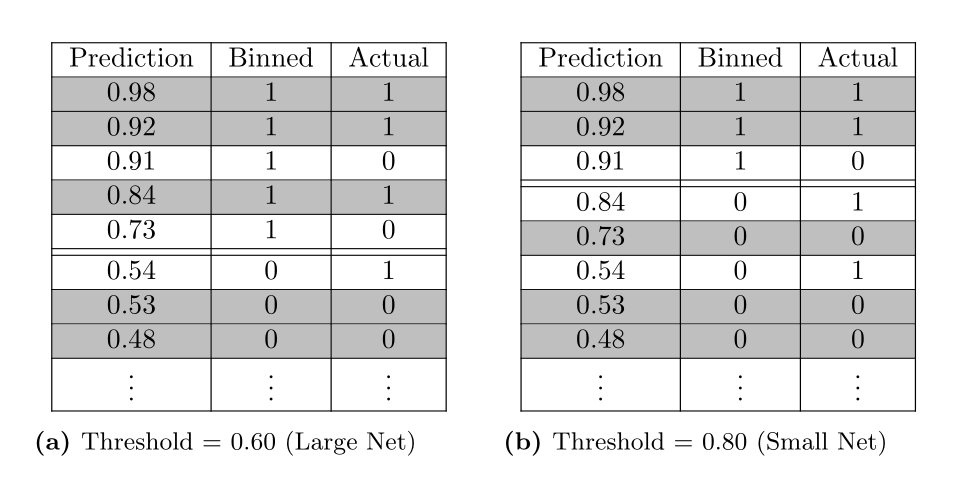
\includegraphics[width=0.9\textwidth]{Fig3.png} %TODO: REMOVE BEFORE SUBMISSION
    \caption{{\bf Example of two prediction binning thresholds.} The same predictions (Prediction) are binned as a 1 or 0 in the Binned column based on the threshold (represented by the double-horizontal line), then compared to the actual results (Actual) and determined to be correct (gray) or incorrect (no color).}
    \label{fig:threshold_example}
\end{figure}

To provide the HPPs with a large amount of information in a concise form, the Receiver Operating Characteristic (ROC) curve is displayed. To create this curve, every possible binning threshold is chosen, the binned predictions are evaluated against the ground truth known outcomes, then FPR and TPR are calculated. The FPR and TPR paired values are plotted as points on the ROC curve~\cite{fawcett2006introduction}.

\subsection*{K-Folds}
It is standard practice in data science to test prediction models by fitting them to a set of data, use them to predict on data they have not yet seen, then only evaluate whether the predictions were correct on this previously unseen dataset. This is achieved in practice by selecting a random subset of the data and saving it apart from the rest to be used for testing after the model is trained. This subset of data is referred to as the ``test set.'' The remaining data is called the ``training set'' because this is the data with which the model is fit, or ``trained.'' 

K-Folds is a model evaluation technique where the data is split into $k$ disjoint groups, or folds. A loop is run where the model is trained and tested on different splits of the data; a different split for each fold. For each fold, one of the data subsets is saved as the test set and the remaining folds become the training set. The model is trained and evaluated on this data split, then the whole process is repeated using the next fold as the test set. We used $k = 10$ folds, which is the default number of folds suggested in the literature~\cite{marcot2020optimal}.

The model evaluation metrics are calculated on the combined predictions of all the folds so are the average over all of these data splits. In this way the model is always evaluated on data it has not yet seen and the resulting averaged evaluation metrics are less sensitive to each individual train-test split. Also, the combined predictions from all the model runs cover the entire dataset, so every person's outcome is predicted.

\subsection*{Sampling and scaling}
% Oversampling
The method of naive random oversampling the minority class (positives) was employed to combat the extreme imbalance in the dataset. Once the data split for each fold was performed, the training set was balanced by oversampling the minority class until the number of positives and negatives was the same. The test set was not oversampled for any fold.

In order to make the model parameters easily comparable, the method of min-max scaling was performed for each fold. After the data split was performed for each fold, the data was scaled using Eq~\ref{eq:minmaxscale} for feature $i$ and data point $j$, so that all the values for feature $i$ fall within the new range of [0, 1]. The min and max of feature $i$ are found in the training set of each fold and then the scaling process is applied to both the training and test sets of each fold.

\begin{equation}
    \centering
    x_{i, \hat{j}} = \frac{x_{i, j} - \text{min}(x_{i})}{\text{max}(x_{i}) - \text{min}(x_{i})}
    * (1 - 0) + 0
    \label{eq:minmaxscale}
\end{equation}

%------------------- RESULTS ---------------------------------
\section*{Results}
The method of K-Folds was employed with $k=10$, so ten separate models were actually trained and act as an ensemble model in practice. The reported performance is an average of all the individual models. If similar performance is to be attained on new data, all models must predict the risk of experiencing homelessness for a new person, the maximum predicted risk must be taken from each model, then these model maximum predictions must be averaged to produce the overall prediction for each person. This follows the same procedure as performed in model evaluation.

In order for the model to be applied in practice, a specific binning threshold must be chosen with different thresholds yielding different model performances. The appropriate threshold will depend upon the relative costs of FPs to FNs in the specific context the prediction is being performed. For example, if a HPP uses an expensive intervention, the cost of FPs can be large, so a high threshold with few FPs is preferred, but if an inexpensive intervention is used in the same context the cost of FPs is smaller so a lower threshold that correctly identifies more positives is preferred. High thresholds correspond to the lower left region of the ROC plot (Fig~\ref{fig:ROC}) where the TPR and the FPR are both low because few people are predicted as positive. \red{reduce or remove paragraph?}

\begin{figure}[htb]
    \centering
    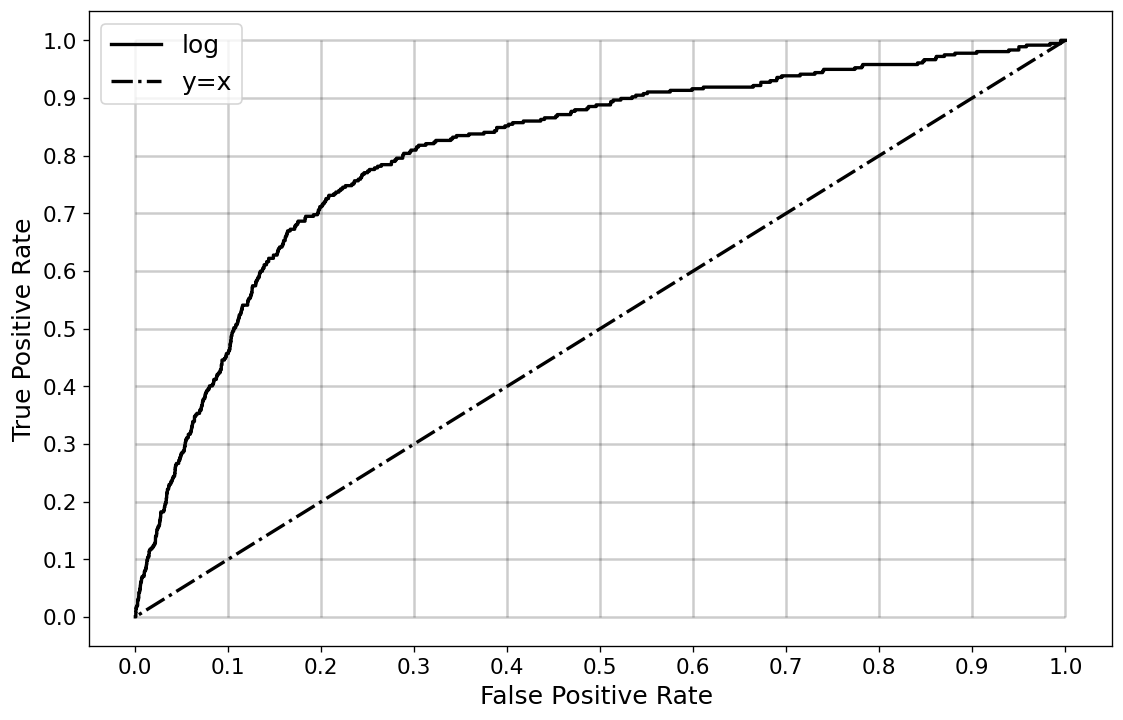
\includegraphics[width=\textwidth]{Fig4.png} %TODO: REMOVE BEFORE SUBMISSION
    \caption[ROC curve]{{\bf The ROC curve for the Logistic Regression Model.} This plot is created by choosing every possible binning threshold, then at each threshold evaluating FPR and TPR. The plot consists of only the (FPR, TPR) points. FPR (False Positive Rate) is the proportion of false positives to total ground truth negatives. TPR (True Positive Rate) is the proportion of true positives to the total ground truth positives. AUC (Area Under the Curve) is 0.808.}
    \label{fig:ROC}
\end{figure}

The coefficient for each feature shown in Table~\ref{tbl:meanParams} provides a measure of the feature's importance to the logistic model. A feature with a coefficient further from zero means the model gives that feature more weight when computing the prediction. From Table~\ref{tbl:meanParams} we can see that NUM\_PREM\_FOR\_PER and BREAK\_ARRANGEMENT are by far the most important features, PAST\_DUE moderately influences model predictions, and TOTAL\_CUR\_BALANCE and NUM\_PER\_FOR\_PREM are much less important to the model. This direct comparison is only possible with data scaled to the same range. With unscaled data, the odds ratio describes how much the predicted odds of an event will increase if a single variable is increased by one, but is meaningless with scaled data because the increase of one occurs in the scaled range, not the original data range. 

\begin{table}[!h]
    \centering
    \begin{tabular}{lcccc}
    \toprule
    Feature &                    Coeff &       [0.025 &       0.975] &  OR \\
    \midrule
             PAST\_DUE &         0.406 &        0.405 &        0.407 &    1.501 \\
    TOTAL\_CUR\_BALANCE &        0.001 &        0.001 &        0.001 &    1.001 \\
     NUM\_PREM\_FOR\_PER &      -0.991 &       -0.995 &       -0.988 &    0.371 \\
    BREAK\_ARRANGEMENT &         0.803 &        0.789 &        0.816 &    2.231 \\
     NUM\_PER\_FOR\_PREM &       0.078 &        0.075 &        0.080 &    1.081 \\
    \bottomrule
    \end{tabular}
    \caption{{\bf Model parameters.} Mean logistic model coefficient (Coeff), mean 95\% confidence interval for the coefficient for each model feature, and mean odds ratio (OR) over all folds. The relative importance of the features can be determined by examining their model coefficients.}
    \label{tbl:meanParams}
\end{table}

The sign of each model coefficient also provides information; a positive coefficient means that an increase in the feature causes an increased predicted risk, while a negative coefficient means an increase in the feature causes a decreased predicted risk. From Table~\ref{tbl:meanParams}, an increase in all features causes an increase in predicted risk, except for NUM\_PREM\_FOR\_PER where an increase in this feature causes a decrease in predicted risk.

In order to make the results of this study comparable to other homelessness prediction studies, the results of our model evaluated at the threshold where the TPR is near the levels listed in the other studies are shown in Table~\ref{tbl:performance}. Each row in Table~\ref{tbl:performance} represents a single (FPR, TPR) point on the ROC curve in Fig~\ref{fig:ROC}. Most of the points plotted in on the ROC curve are not tabulated, but an overall sense of performance can be obtained for all thresholds using only the ROC plot.

\begin{table}[htb]
    \centering
    \begin{tabular}{ccccccc}
        \toprule
        Threshold   &   TPR &   FPR & PPV   & Accuracy  &  Balanced Accuracy    & F-1 Score \\
        \midrule
        0.559       & 0.776 & 0.252 & 0.012 &     0.748 &     0.762             & 0.023 \\
        0.500       & 0.818 & 0.307 & 0.010 &     0.693 &     0.755             & 0.020 \\
        0.407       & 0.899 & 0.522 & 0.007 &     0.480 &     0.689             & 0.013 \\
        0.378       & 0.922 & 0.664 & 0.005 &     0.338 &     0.629             & 0.011 \\
        \bottomrule
    \end{tabular}
    \caption{{\bf Selected thresholds and their corresponding performance metrics.} These (FPR, TPR) points are displayed in the ROC plot shown in Fig~\ref{fig:ROC}. TPR (True Positive Rate) is also referred to as Sensitivity, Recall, and Hit Rate. FPR (False Positive Rate) is also referred to as Fallout Rate. PPV (Positive Predictive Value) is also referred to as Precision.}
    \label{tbl:performance}
\end{table}

%------------------- DISCUSSION ---------------------------------
\section*{Discussion}
\subsection*{Model performance}
Performance of models intended for a specific use, such as homelessness prediction, is most useful when analyzed and presented in a manner convenient for the intended users of the models. In this case the intended users are HPPs, so the performance of this model is presented in a manner conducive to an HPP selecting a prediction model for their particular situation.

Comparing binary classification models is difficult because their scores in performance metrics differ based on the chosen prediction binning threshold. Model performance encompasses how accurately the model predicts positive cases and negative cases. These are both driven by the chosen threshold, but typically the relationship between the threshold and model performance is not straightforward, meaning as the threshold is changed there is no predictable way in which true/false positives/negatives will change. This complicated relationship between threshold and model performance causes difficulty in model comparison. For instance, Model A may perform better than Model B at one threshold, but Model B performs better at another threshold. Additionally, at a single threshold, Model A may perform better than Model B in one metric, but worse in another metric. The most helpful way to compare models may be to compare only their performances on positive and negative cases without considering the threshold at all; the threshold can be treated as a model parameter.

Because in this use-case it is much worse to incur a Type II Error (false negative) than a Type I Error (false positive), we present model performance and evaluation at a threshold where the TPR is high, meaning most of the positive cases are correctly predicted. This focus on correctly predicting positive cases has been repeatedly pointed out in the literature~\cite{vanberlo2021interpretable,hong2018applications}. We chose to report the prediction binning threshold that produces a TPR as near to 0.90 (90.0\%) as possible, then report FPR and other metrics at the same threshold. Reporting the FPR allows homelessness prediction programs to assess the costs and savings of the prediction model based on their service population.

\subsubsection*{Comparison with current research}
We compare our model to those developed in previous studies by choosing the prediction binning threshold that produces most closely the same TPR as reported by each of the previous studies, then comparing the FPRs or PPVs, when provided. For the same TPR a lower FPR and higher PPV are preferred. Several studies presented their model performance in ways, such as plotting an ROC curve or tabulating performance metrics at a TPR of 0.90, allowing for the evaluation of the model at a TPR of 0.90. At a TPR of 0.90, the Cox Proportional Hazards model published by Shinn et al. achieved a FPR of about 0.61~\cite{shinn2013efficient}, the Logistic Regression models of Toros et al. achieved FPRs of 0.297 (unemployed workers model) and 0.364 (youth receiving public assistance model)~\cite{toros2019early}, and the Logistic Regression model of Hong et al. achieved a FPR of about 0.69~\cite{hong2018applications}. At a TPR of 0.889 our model achieved a FPR of 0.522. The machine learning model developed by VanBerlo et al. achieved a TPR of 0.921 and PPV of 0.651 with no FPR reported~\cite{vanberlo2021interpretable}. At the same TPR our model achieved a PPV of 0.005. The Logistic Regression model published by Byrne et al. achieved a TPR of 0.778 with a PPV of 0.117~\cite{byrne2020classification}. At the same TPR our model achieved a PPV of 0.012.

In comparison with the selected studies listed above at the comparable TPR, our model achieved a lower (better) FPR than Shinn's model, a much higher (worse) FPR than either of Toros' models, a lower (better) FPR than Hong's model, a much lower (worse) PPV than VanBerlo's model, and a much lower (worse) PPV than Byrne's model. It is important to note that all studies where model performance was reported - other than Byrne's - were predicting homelessness, return to homelessness, or chronic homelessness based on some subpopulation already seeking government assistance. There is much more relevant data available to predict homelessness on these subpopulations because they have submitted financial, health, employment, etc. information as part of applying for government assistance. These subpopulations also have higher proportions of positive cases, so the data imbalance is less severe.

Byrne's study predicted homelessness on essentially the entire population of Massachusetts using health insurance data. Byrne's is the study most directly comparable to ours, though Byrne's used health data and covered ``more than 98\% of Massachusetts residents''~\cite{byrne2020classification} while our study covered only about 17.5\% of Spokane County residents (based on the 2019 U.S. Census)~\cite{SpokanePop}.

\subsection*{Model parameters}
The model parameters shown in Table~\ref{tbl:meanParams} reveal which features were most important to the model in predicting homelessness and which features, when increased, caused an increased predicted risk. NUM\_PREM\_FOR\_PER (Coeff = -0.991) is the most important feature since it has the greatest magnitude coefficient. BREAK\_ARRANGEMENT (0.803) is the second most important , PAST\_DUE (0.406) the third, NUM\_PER\_FOR\_PREM (0.078) the fourth, and TOTAL\_CUR\_BALANCE (0.001) is the least important.

It is surprising that NUM\_PREM\_FOR\_PER is such an important feature and that it is protective - as the feature increases, the predicted risk of homelessness decreases. This means that if a person has been the main utility account holder at more locations, the model predicts them to be at a lower risk of homelessness. This contradicts the authors' hypothesis that people at risk of homelessness are more transient than the general population and could be due to the upfront costs of moving such as paying rental deposits.

BREAK\_ARRANGEMENT, the number of times an individual has established a service severance with Avista, is clearly a risk indicator. It is interesting that PAST\_DUE, the number of utility bills overdue, is about half as important as BREAK\_ARRANGEMENT in predicting homelessness. This seems to indicate that people at risk of experiencing homelessness may have slightly more bills past due, but are much more likely to establish a service severance with Avista than the general population. 

TOTAL\_CUR\_BALANCE, though the smallest magnitude coefficient, is still helpful in predicting homelessness. This feature coefficient was significantly different from zero and increased model performance.

\subsection*{Data preparation}
\subsubsection*{Including more people per account}
The data preparation scheme associated only the main account holder with each account's billing history and removed all other people associated with the account. This step removes many people from the dataset because they are not a main account holder on any account; 62\% of people are removed during preprocessing, though many of these are removed because their accounts did not exist in the time frame in which billing histories were provided. Ideally as many people as possible would be retained, but testing the inclusion of cotenants and all people associated with an account produced models with much worse performance. This reduced performance is likely due to the account billing history holding little or no information about the financial health of people other than the main account holder.

\subsubsection*{Data homogeneity over time}
For this project, we investigated if the relationships between the predictor variables and the outcome changed over time. The year 2020 was expected to contain different relationships than the previous years because the COVID-19 pandemic caused people and the utility agencies to behave differently than they had in previous years. For example, for the greater part of 2020, the utility agencies that contributed data to our project did not perform service shut-offs as they had in previous years~\cite{white2020utilities}. 

To investigate if there was a difference in the relationships between the variables and the outcome in different years, the data was split by year, the Spearman Correlation of each variable with the outcome (CMIS\_MATCH) was measured, these correlations were then ranked, and the rankings (displayed in Table~\ref{tbl:corr_years}) were compared from year to year. Surprisingly, they are very similar from year to year indicating that the important relationships within the data are similar from year to year. Because of this finding, all available years, 2015 to 2020, were included in modeling. Note that NUM\_PER\_FOR\_PREM and NUM\_PREM\_FOR\_PER do not vary in 2015 because only one month (December) of 2015 was provided, so they have no meaningful correlation with the outcome in that year. It is assumed that NUM\_PER\_FOR\_PREM and NUM\_PREM\_FOR\_PER would be the two highest correlated variables with the outcome if more months from 2015 were provided.

\begin{table}[!h]
    \centering
    \begin{tabular}{lcccccc}
        \toprule
                 Variable &  2015 &  2016 &  2017 &  2018 &  2019 &  2020 \\
        \midrule
        NUM\_PER\_FOR\_PREM &     - &     2 &     3 &     2 &     1 &     1 \\
        NUM\_PREM\_FOR\_PER &     - &     1 &     1 &     1 &     2 &     2 \\
        TOTAL\_CUR\_BALANCE &     3 &     4 &     4 &     4 &     4 &     3 \\
        BREAK\_ARRANGEMENT  &     4 &     3 &     2 &     3 &     3 &     4 \\
        PAST\_DUE           &     5 &     5 &     5 &     5 &     5 &     5 \\
        \bottomrule
    \end{tabular}
\caption{{\bf Correlation by year.} Ranks of Spearman Correlation between each predictor and the outcome, by year. Variables are sorted by 2020 rankings. Since the rankings are very similar from year to year, the relationships between predictor variables and outcome must be similar.}
\label{tbl:corr_years}
\end{table}

\subsubsection*{Other outcomes investigated}
The eventual choice of outcome measure was CMIS\_MATCH, the binary variable corresponding to if a person was ever recorded as experiencing homelessness, but several others were investigated along the way. One was a numerical variable describing the number of months until an individual experienced an episode of homelessness. This approach fits the time series format of the data well and has a clear risk interpretation (closer times are higher risk), but posed the challenge of assigning some value to negative cases. Two more outcomes investigated were the binary variables corresponding to if an individual was within six months or one month of experiencing an episode of homelessness.

The outcome used for modeling, CMIS\_MATCH, was chosen because out of the potential outcome measures it was the most closely associated with the predictor variables. It is surprising that the outcomes corresponding to if an individual will experience homelessness within six months and one month are associated less with the predictor variables than CMIS\_MATCH. This seems to indicate that the data used for this project is better at discerning if an individual will ever experience homelessness than it is at discerning either if the individual will experience homelessness within the month or within six months.

\subsection*{Dependence on time}
It was hypothesized that time is an important factor in predicting homelessness. As people get closer in time to experiencing homelessness they are thought to be more distinguishable from the general population of mostly negative cases. Two approaches were considered to incorporate individual's previous characteristics in predicting the likelihood of homelessness.

The first approach was to generate simple trajectories for each person over time. This was done by fitting a linear line for each variable over time, then retaining only the slope of the line instead of the original values. This method records the long-term trend of a person in each variable over time. Another method investigated was to take the difference between months for each variable. These differences capture the local changes in people's characteristics and were used as predictors in the place of the original variable values. Model performance was worse for these two approaches than for the methods described for this project.

The highest performing method investigated was to treat each person-place-month combination as a separate entity, make a prediction for each entity, then take the maximum risk prediction for each person over all places and months that person appears in the dataset. This is the method used and described in the Methods Section and seems to indicate the important aspect of each person is their peak risk. 

Two versions of Cox Regression, Cox Proportional Hazards and Cox Time Varying Covariates, were investigated. Cox Proportional Hazards did not fit the situation because here the risk of experiencing homelessness depends upon the characteristics of each individual, which change over time. Cox Time Varying Covariates was found to perform essentially the same task as our Logistic Regression approach in this context. Additional methods appropriate to prediction on time-series data should be investigated for application in this context. 

\subsection*{Data limitations - summary}
An expanded version of this section is available in the Supporting Information Section. There are two main limitations to the utility billing data used for this project: lack of coverage and uncertainty in negative labels. The data was chosen because it was thought to contain financial health information on the general population, but because account histories only provide information on the main account holder, only about 17.5\% of the total Spokane County population was represented in the data~\cite{SpokanePop}.

The other major limitation to the data was uncertainty in the negative outcome labels. Positive labels have a high confidence in correctness - people labeled as positive almost certainly did seek assistance at the times recorded. Some people labeled as negative, though, likely did experience homelessness but were simply never recorded. This is an unknown factor in the data and may have negatively impacted model performance.

Model performance would likely improve if additional data sources were leveraged, such as those used by previous research: physical health, mental health, criminal justice, job related, etc.

%------------------- CONCLUSION ---------------------------------
\section*{Conclusion}
By creating a prediction model based on residential utility customer billing information, we showed that this data is useful for predicting homelessness. The data is ubiquitous across the United States and contains financial health information, but does not cover the entire population. The model produced for this project has performance similar to the current research while predicting on the general population, not just those seeking assistance.

%------------------- SUPPORTING INFORMATION ---------------------------------
\section*{Supporting information}
\subsection*{Data limitations - extended}
\subsubsection*{Incompleteness and data integrity}
% Incompleteness of data: small part of population
The first limitation is the incompleteness of the data; only a small portion of the overall population was represented. The utility billing data was structured to track accounts and ensure the people responsible for those accounts paid their bills on time. The data captures 91,591 people, only 17.5\% of the total Spokane County population which was recorded by the U.S. Census to be 522,798 in 2019~\cite{SpokanePop}. Though the billing data does appear to contain useful information related to homelessness, other sources of financial data may have better coverage.

% Incompleteness of data: don't know who paid bills
There were often multiple people associated with a single utility account, but it was not recorded who paid for each bill. For this project it was assumed that the main account holder always paid since they were ultimately financially responsible for the account, but this may not always have been the case. There may be useful information regarding who paid a utility bill for each month; specifically, it may be a risk indicator for the main account holder if someone other than the main account holder paid the bill for a given month. It also may be a positive financial health indicator for the bill payer.

% Matching: don't know who pays bills
The question of who paid each utility bill is made more difficult to answer by the fact that Avista and City utility billing information was matched using address, not person. This choice was made because matching on address and month across the billing systems of Avista and the City of Spokane had a much higher match rate than matching on the recorded account holder names. It is likely that many of the City utility bills for apartments were paid by the landlord and so would remain unaltered if the tenant was experiencing financial stress. This aspect is addressed, to some degree, by the selection of explanatory variables. It was found that the aggregated measure TOTAL\_CUR\_BALANCE, the combined amount owed to Avista and the City, was most associated with the outcome measure over the amounts owed to the individual entities. This indicates that even if many landlords did pay for the City utilities, even for people who were at risk of homelessness, there was enough information in the amounts owed in City utilities regarding homelessness that aggregating the Avista and City amounts owed produced a variable more strongly associated with CMIS\_MATCH than the individual variables.

% Mislabeled negative cases
Another important limitation of the data is our confidence in the accuracy of the outcome labels. Of all the people in the data labeled as positive, our confidence that they are actually positive is high - they matched someone who was recorded as experiencing homelessness in the Spokane area. Our confidence in the correct labeling of the negative cases, on the other hand, is lower. Some cases labeled as negative in the data may, in reality, be positive cases if they did experience homelessness, but this fact was not recorded in the City of Spokane CMIS database. This might have occurred if someone experiencing homelessness did not seek assistance or if they moved away from the Spokane area before seeking assistance based on their homelessness status. Because some cases labeled as negative may be positive cases in reality, model performance may appear worse than it actually is. This problem is likely common to the task of predicting homelessness.

% Mislabeled positive cases: not first-time homelessness
In addition to potentially mislabeled negatives, the labeled positives may not correspond to first-time homelessness. In the preprocessing step, in an effort to capture first known homelessness episode, only data recorded prior to service seeking for positive cases was retained. However, individuals may have experienced homelessness prior to the study period in Spokane County or elsewhere. This may not be of import if the prediction task is reframed as a method to identify the pattern of first-time homelessness. With this view people who have experienced homelessness in the distant past may present the same pattern of experiencing a new episode of homelessness as another person would in experiencing first-time homelessness. This area may require further study and would benefit from a national homelessness database to help distinguish between first-time homelessness and repeat homelessness.

\subsubsection*{Other related outcomes}
% Predictions related to other outcomes
A point of interest is that the people predicted as positive by the models may be members of a more general at-risk population. The only outcomes we had data on were related to homelessness, but the model predictions and the data investigation reveal that many people labeled as negatives have similar characteristics to the positive cases. These false positives may be financially stressed or at-risk in ways other than their housing status, but we did not have data on other types of outcomes to investigate this. One study that investigated both homelessness and drug addiction found that ``predicted homeless status was associated with a nearly 23-fold increase in the risk of fatal opioid overdose''~\cite{byrne2020classification}. One approach may be to create a tiered screening model system, starting with a model that predicts general risk, and progressing to models that predict more and more specific service needs.

\subsubsection*{Challenges utilizing location information}
% Challenges including location in model
Variables related to housing and location were hypothesized to be important predictors of homelessness, but were challenging to include as predictors in the model. Information such as rent, desirability of living location, and age and condition of residence are likely related to an individual's financial health and therefore be good predictors of homelessness. The variables available that contain geographical location information were POSTAL, the person's postal code, BLOCKGROUP\_GEOID, the U.S. Census block group number, and SPA\_PREM\_ID, the assigned identification number for a specific residence. The unit of block group is smaller than that of postal code, but block group areas often do not fall within a single postal code boundary. All of these variables are categorical with POSTAL having 17 unique levels represented in the data, BLOCKGROUP\_GEOID having 279, and SPA\_PREM\_ID having 64,728. Because BLOCKGROUP\_GEOID and SPA\_PREM\_ID had so many possible values, they could not be incorporated into the logistic regression model without causing convergence issues. POSTAL was too general to have much meaningful information regarding such a rare event as homelessness. 

% Other location-based approaches
Other approaches to incorporating location information as a predictor should be investigated. Some prior analysis could be performed to determine at-risk areas such as low-rent and subsidized rent areas. These could be represented in a few-leveled categorical variable. Individuals in the study could be determined to reside in one or none of these areas.

\subsubsection*{Additional data}
% Additional information more related to homelessness
There is other information closely related to homelessness that we did not utilize for this study. Other studies have found that income, health services usage, criminal justice system interaction, and government assistance usage all contain useful information for predicting homelessness~\cite{byrne2020classification,flaming2011crisis,hong2018applications,shinn2013efficient,vanberlo2021interpretable}. Income, or financial health, we hypothesize is an especially useful predictor for homelessness, but it is difficult to acquire such data on the general population to predict homelessness at the population scale. We hoped to fill that knowledge gap using the proxy of customer utility billing information. A model constructed using a combination of all these data sources (financial health, physical and mental health, criminal justice, etc.) would likely have far superior performance. 

\subsection*{Project code}
All code related to this project is freely available at the following GitHub repository:  
\url{https://github.com/middlec000/SPA_predict_homelessness}

%------------------- ACKNOWLEDGEMENTS ---------------------------------
\section*{Acknowledgements}
This project is a result of the combined efforts of the member organizations of the Spokane Predictive Analytics group: Avista Utilities, the City of Spokane, Urbanova, and Eastern Washington University. Avista Utilities and the City of Spokane provided data and specialized knowledge, the Avista data team provided initial data matching and de-identification, Urbanova provided data hosting, and Eastern Washington University provided analysis and predictive modeling. This project would not be possible without the cooperation and support of all organizations.

\nolinenumbers

% Either type in your references using
% \begin{thebibliography}{}
% \bibitem{}
% Text
% \end{thebibliography}
%
% or
%
% Compile your BiBTeX database using our plos2015.bst
% style file and paste the contents of your .bbl file
% here. See http://journals.plos.org/plosone/s/latex for 
% step-by-step instructions.
% 

%%   Temporary Bibfile included here

\bibliography{PLOS_ONE_MO_Bibliography.bib}
\bibliographystyle{plos2015.bst}

\end{document}
